\chapter{Introduction}
\label{chap:intro}
%http://thesistips.wordpress.com/2012/03/25/how-to-write-your-introduction-abstract-and-summary/

% It introduces the problem and motivation for the study.
When located in an unknown area, it can be useful to have information about the area around you. Examples of this could be map data for navigation, plans for public transport in the area or locations of nearby restaurants. It is usually possible to retrieve this kind of data using a smart phone with a mobile Internet connection. Data connections can however not be trusted to be available everywhere. This could be a concern for someone traveling in an area they haven't visited before.

An example of potential connection problems can be seen in figure \ref{fig:coveragemap}.
The map displays a screenshot of a coverage map, showing a few problematic areas, especially north of Aars. The coverage is that of the telephone company TDC hosted on their website\cite{tdccoverage}. Speeds of "Up to 0,2 mbit" are not shown as it can not be considered a reliable data connection (up to 0,2 can also be 0). There are however further issues than shown directly on the map.

By TDC's own description (translated): "The speeds displayed on the coverage map is derived from a calculation of plausible speed, not a measure of actual speeds. The measure takes into account the altitude of the masts and altitude differences in the terrain."
While this makes sense, it also means that obstructions (other than terrain) has not been considered for the map. Adding these in could make the map even worse, as mentioned on the TDC webpage: "(...) If one is outside the building, trees and surrounding buildings can also attenuate the speed, but typically not in the same amount".
To make it even worse the displayed speeds are only with 70\% certainty: "The displayed speeds shows the expected capacity for the majority of use ($\sim$70\%)."

Adding all these considerations into the map, it is obvious that a real-time coverage map would not match the theoretical model. 

\begin{figure}[H]
\centering
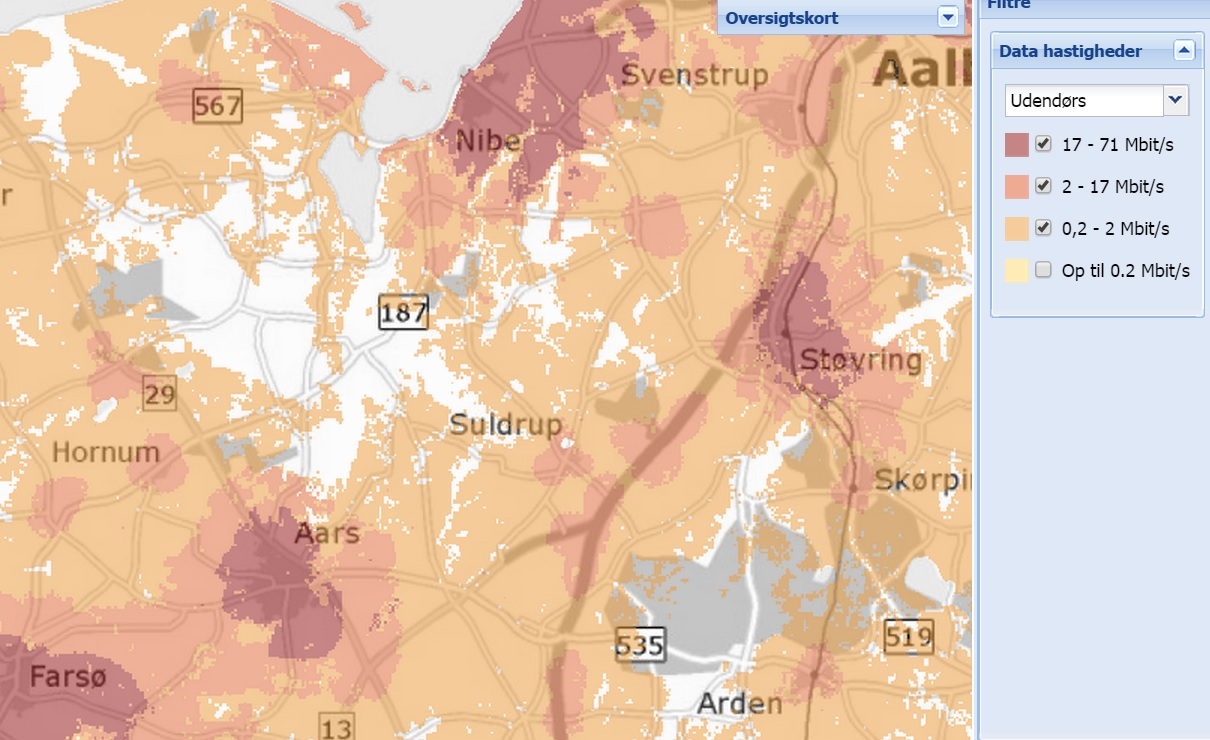
\includegraphics[width=\textwidth]{billeder/coverage}
\caption{Example of missing coverage}\label{visina8}
\label{fig:coveragemap}
\end{figure}

Regardless the state of available connections, it would be ideal to always have relevant data on the phone. This would however require that one can predict when to get the data, before the connection drops out. As a user it is possible to download these data manually, but also impractical as it would require manual monitoring of the signal strength. Furthermore it would require some effort to continuously update the phone with all the relevant data. It would be ideal if the smart phone could handle it automatically.



% - Tell the reader what the topic of the report is.
% - Explain why this topic is important or relevant.

% It provides a brief summary of previous engineering and/or scientific work on the topic.
% - Here you present an overview what is known about the problem.  You would typically cite earlier studies conducted on the same topic and/or at this same site, and in doing so, you should reveal the yawning void in the knowledge that your brilliant research will fill.

% It outlines the purpose and specific objectives of the project.

% It provides a ‘road map’ for the rest of the report.
% - This is so that the reader knows what’s coming and sees the logic of your organization.
% - Describe (in approximately one sentence each) the contents of each of the report/thesis chapters.
\section{Roadmap}
The following is a brief description of each chapter in the report

% add more here as report progresses %
\subsection{Design and Implementation}
\subsection{Test}
\subsection{Future Work}
\subsection{Conclusion}